\section{Commonly used \LaTeX\  features}

This section includes a few examples of \LaTeX\  components you can reuse in your thesis. See the \texttt{example.tex} file for the source code of this section.

\subsection{Citations and references}
Citations are imporant part of scientific papers and theses. In \LaTeX\  you first have to label and list the works you want to cite in the bibliography section (see \texttt{biblio.tex}), and then you can refer to them anywhere in the document by using this label, like this~\cite{erlangdocs}. If you want to cite more than one work, you can cite them like this~\cite{refactorerl1, refactorerl2}.

A different type of label definition can also be used to refer to certain parts of the documents, like figures (see Section \ref{sec:fig}.), and chapters, sections, subsections. Chapter labels can also be utilized to refer to an appendix (like Appendix \ref{apx:example}). 

\subsection{Mathematics}
Representing mathematical formulas is one of the strongest suits of \LaTeX.

Inline formula: $x^2 + y^2 = z^2$. This is also useful to write single mathematical symbols, like $\alpha$ or $\implies$ or $\leftarrow$.

Standalone formula:
$$ x^2 + y^2 = z^2 $$

Numbered formulas:
\begin{equation}
x^2 + y^2 = z^2
\end{equation}
\begin{equation}
\binom{n}{k} = \frac{n!}{k!(n-k)!}
\end{equation}

Aligned formulas:
\begin{align}
x^2 + y^2 &= z^2 \\
\binom{n}{k} &= \frac{n!}{k!(n-k)!}
\end{align}

Aligned unnumbered formulas:
\begin{align*}
x^2 + y^2 &= z^2 \\
\binom{n}{k} &= \frac{n!}{k!(n-k)!}
\end{align*}

\begin{mydef}
A graph is an ordered pair $G = (V, E)$ comprising a set $V$ of vertices, nodes or points together with a set $E$ of edges, arcs or lines, which are 2-element subsets of $V$ (i.e., an edge is associated with two vertices, and the association takes the form of the unordered pair of the vertices).
\end{mydef}

\begin{myexamp}
Let $V$ and $E$ be the sets
\begin{align*}
V &= \{1, 2, 3, 4, 5, 6\} \\
E &= \{\{1, 2\}, \{1, 5\}, \{2, 3\}, \{2, 5\}, \{3, 4\}, \{4, 5\}, \{4, 6\}\}
\end{align*}
Then $(V,E)$ is a graph.
\end{myexamp}

\subsection{Figures}
\label{sec:fig}
You can include, resize, and position figures using the figure environment and the \texttt{includegraphics} directive. This environment makes it possible to add captions to a figure, and to add a custom label by which you can refer to this figure anywhere in the document. See the Latex source of Figure \ref{fig:ecore} in \texttt{examples.tex}. To include big figures, you can rotate the image with the \texttt{sidewaysfigure} environment, as in the case of Figure \ref{fig:omgfsm}.
\begin{figure}[h]
\centering
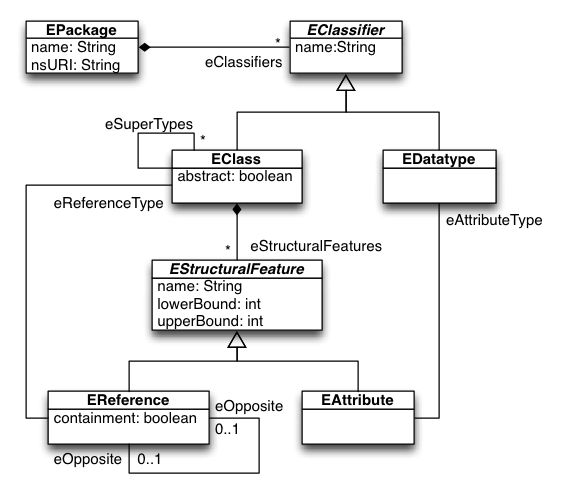
\includegraphics[width=.7\textwidth]{figures/ecore.png}
\caption{A small image, centered horizontally~\cite{ecore}.}
\label{fig:ecore}
\end{figure}

\begin{sidewaysfigure}
\centering
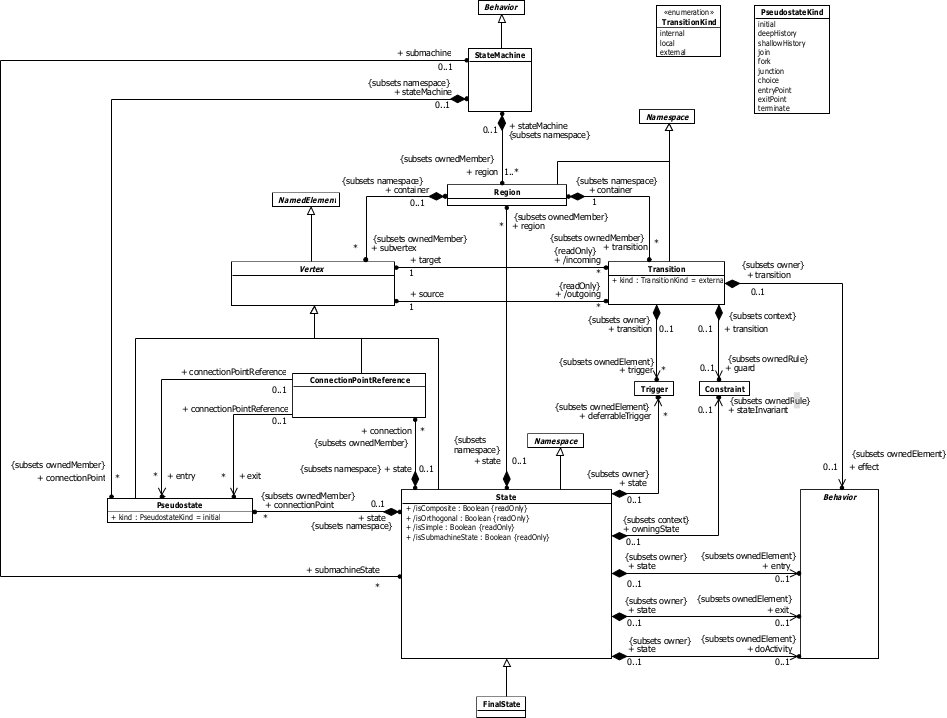
\includegraphics[width=\maxwidth{\textwidth}]{figures/omgfsm.png}
\caption{A wholepage image, rotated sideways~\cite{omguml}.}
\label{fig:omgfsm}
\end{sidewaysfigure}

\subsection{Diagrams}
It's also possible to draw diagrams \textit{inside} \LaTeX\ code.
\[
\begin{tikzcd}
L\arrow{d}{tr} = & (L^S \arrow{d}{tr^S} &   \arrow{l}{s_L}  L^C\arrow{d}{tr^C} \arrow{r}{t_L} & L^T \arrow{d}{tr^T}) \\
R = & (R^S & \arrow{l}{s_R} R^C \arrow{r}{t_R} & R^T)
\end{tikzcd}
\]

\clearpage
\subsection{Lists}
List for unordered things:
\begin{itemize}
\item Apple is a deciduous tree in the rose family best known for its sweet, pomaceous fruit, the apple.
\item Orange is the fruit of the citrus species Citrus $\times$ sinensis in the family Rutaceae. The fruit of the Citrus $\times$ sinensis is considered a sweet orange, whereas the fruit of the Citrus $\times$ aurantium is considered a bitter orange.
\item Pomegranate is a fruit-bearing deciduous shrub or small tree in the family Lythraceae that grows between 5 and 8 m tall.
\end{itemize}

Enumerated list for ordered things:
\begin{enumerate}
\item Open door.
\item Enter room.
\item Close door. 
\end{enumerate}

Named list for dictionary-like descriptions:
\begin{description}
\item[Apple] A deciduous tree in the rose family best known for its sweet, pomaceous fruit, the apple.
\item[Orange] The fruit of the citrus species Citrus $\times$ sinensis in the family Rutaceae. The fruit of the Citrus $\times$ sinensis is considered a sweet orange, whereas the fruit of the Citrus $\times$ aurantium is considered a bitter orange.
\item[Pomegranate] A fruit-bearing deciduous shrub or small tree in the family Lythraceae that grows between 5 and 8 m tall.
\end{description}

\subsection{Text formatting}
The usual text formatting options (\textbf{bold}, \textit{italic}, \texttt{fix-width}) are also available in \LaTeX. 
\begin{verbatim}
The verbatim environment can be used to
present multiline text with fix-width font.
\end{verbatim}

\clearpage
\subsection{Algorithm}
Below is an example usage of the algorithm environment. You can use this environment to include pseudocode in your thesis, usually to describe programs and algorithms you invented.


\algdef{SE}[DOWHILE]{Do}{doWhile}{\algorithmicdo}[1]{\algorithmicwhile\ #1}%
\begin{algorithm}
\footnotesize
\caption{$discoverGenFsm(modulName)$}         
\label{dfs}                           
\begin{algorithmic}[1]
  \State $ spgModel \leftarrow new SpgModel()$
  \State $ root \leftarrow new Root()$
  \State $ spgModel.setRoot(root) $
  \State $ modul \leftarrow new Modul(modulName) $
  \State $ root.addChild('mod', modul) $
  
  \For{$ f \in initFuns$ }
      \State $modul.addChild('func', erlNode2ModelNode(f))$
   \EndFor 

  \State $ visited \leftarrow new Set(initFuns) $
  \State $ stack \leftarrow new Stack(initFuns) $

  \State $ Visited \leftarrow Init$
  \State $S \leftarrow stack(V)$

  \While{ $stack \neq \varnothing$ } 
    \State $ node \leftarrow stack.pop()$

    \If {$v \not\in visited$}
      \State $ visited.add(node)$
      \State $ modelNode \leftarrow erlNode2ModelNode(node)$
      \State $ neighbours \leftarrow nextNode(node) $
      \For{$ (e,n) \in neighbours$ }
        \State $stack.add(n)$
        \State $modelNode.addChild(e, erlNode2ModelNode(node))$
      \EndFor 
    \EndIf
  \EndWhile    

  \Return $spgModel$
\end{algorithmic}
\end{algorithm}


\subsection{Source code}
Below is an example usage of the listings environment. You can use this environment to include source code in your thesis, usually to show source code examples.   

\begin{figure}[h]
\begin{lstlisting}[extendedchars=true, language=Erlang, basicstyle=\footnotesize\ttfamily, keywordstyle=\color{red}]
-module(hello). 
-export([hello_world/0]).

%% Outputs "hello world\n" on the standard output.
hello_world(ok) ->   
    X = "hello world\n",  
    io:fwrite(X); 

hello_world(_) ->  
   ok. 
\end{lstlisting}
\caption{A "Hello world" program in the Erlang language. Syntax highlighting is provided by the listings environment.}
\label{fig:helloworld}
\end{figure}

\subsection{Tables}
\begin{table}[!htb]
\centering
    \caption{Runtime test results}
    \label{tab:tests}
\noindent\adjustbox{max width=0.9\textwidth}{
    \begin{tabular}{|c|c|c|}
    \hline
    \textbf{Module}              & \textbf{Line no.}   & \textbf{Average (ms)}\\
    \hline
    \multicolumn{3}{|c|}{Ejabberd}                                            \\
    \hline
    ejabberd\_c2s                & 3128                & 31614.7              \\
    \hline                                                                    
    ejabberd\_service            & 404                 & 17991.3              \\
    \hline                                                                    
    eldap                        & 1196                & 27353.0              \\
    \hline                                                                    
    mod\_proxy65\_stream         & 291                 & 14975.9              \\
    \hline                                                                    
\multicolumn{3}{|c|}{Riak}                                                    \\
    \hline                                                                    
    riak\_kv\_2i\_aae            & 695                 & 11688.4              \\
    \hline                                                                    
    riak\_kv\_get\_fsm           & 787                 & 5521.9               \\
    \hline                                                              
\multicolumn{3}{|c|}{Erlang OTP}                                              \\
    \hline                                                              
    ssh\_connection\_handler     & 1721                & 67467.6              \\
    \hline                                                               
    tls\_connection              & 975                 & 56788.5              \\
    \hline
    \end{tabular}}
\end{table}

